\documentclass[]{book}
\usepackage{lmodern}
\usepackage{amssymb,amsmath}
\usepackage{ifxetex,ifluatex}
\usepackage{fixltx2e} % provides \textsubscript
\ifnum 0\ifxetex 1\fi\ifluatex 1\fi=0 % if pdftex
  \usepackage[T1]{fontenc}
  \usepackage[utf8]{inputenc}
\else % if luatex or xelatex
  \ifxetex
    \usepackage{mathspec}
  \else
    \usepackage{fontspec}
  \fi
  \defaultfontfeatures{Ligatures=TeX,Scale=MatchLowercase}
\fi
% use upquote if available, for straight quotes in verbatim environments
\IfFileExists{upquote.sty}{\usepackage{upquote}}{}
% use microtype if available
\IfFileExists{microtype.sty}{%
\usepackage{microtype}
\UseMicrotypeSet[protrusion]{basicmath} % disable protrusion for tt fonts
}{}
\usepackage{hyperref}
\hypersetup{unicode=true,
            pdftitle={Hizkuntzaren Didaktika (Lehen Hezkuntza)},
            pdfborder={0 0 0},
            breaklinks=true}
\urlstyle{same}  % don't use monospace font for urls
\usepackage{natbib}
\bibliographystyle{apalike}
\usepackage{longtable,booktabs}
\usepackage{graphicx,grffile}
\makeatletter
\def\maxwidth{\ifdim\Gin@nat@width>\linewidth\linewidth\else\Gin@nat@width\fi}
\def\maxheight{\ifdim\Gin@nat@height>\textheight\textheight\else\Gin@nat@height\fi}
\makeatother
% Scale images if necessary, so that they will not overflow the page
% margins by default, and it is still possible to overwrite the defaults
% using explicit options in \includegraphics[width, height, ...]{}
\setkeys{Gin}{width=\maxwidth,height=\maxheight,keepaspectratio}
\IfFileExists{parskip.sty}{%
\usepackage{parskip}
}{% else
\setlength{\parindent}{0pt}
\setlength{\parskip}{6pt plus 2pt minus 1pt}
}
\setlength{\emergencystretch}{3em}  % prevent overfull lines
\providecommand{\tightlist}{%
  \setlength{\itemsep}{0pt}\setlength{\parskip}{0pt}}
\setcounter{secnumdepth}{5}
% Redefines (sub)paragraphs to behave more like sections
\ifx\paragraph\undefined\else
\let\oldparagraph\paragraph
\renewcommand{\paragraph}[1]{\oldparagraph{#1}\mbox{}}
\fi
\ifx\subparagraph\undefined\else
\let\oldsubparagraph\subparagraph
\renewcommand{\subparagraph}[1]{\oldsubparagraph{#1}\mbox{}}
\fi

%%% Use protect on footnotes to avoid problems with footnotes in titles
\let\rmarkdownfootnote\footnote%
\def\footnote{\protect\rmarkdownfootnote}

%%% Change title format to be more compact
\usepackage{titling}

% Create subtitle command for use in maketitle
\providecommand{\subtitle}[1]{
  \posttitle{
    \begin{center}\large#1\end{center}
    }
}

\setlength{\droptitle}{-2em}

  \title{Hizkuntzaren Didaktika (Lehen Hezkuntza)}
    \pretitle{\vspace{\droptitle}\centering\huge}
  \posttitle{\par}
    \author{true}
    \preauthor{\centering\large\emph}
  \postauthor{\par}
      \predate{\centering\large\emph}
  \postdate{\par}
    \date{2019/2020}

\usepackage{booktabs}
\usepackage{amsthm}
\usepackage[basque]{babel}
\makeatletter
\def\thm@space@setup{%
  \thm@preskip=8pt plus 2pt minus 4pt
  \thm@postskip=\thm@preskip
}
\makeatother

\begin{document}
\maketitle

{
\setcounter{tocdepth}{1}
\tableofcontents
}
\hypertarget{ikasgaia-hizkuntzaren-eta-literaturaren-didaktika---25868}{%
\chapter*{Ikasgaia Hizkuntzaren eta Literaturaren Didaktika - 25868}\label{ikasgaia-hizkuntzaren-eta-literaturaren-didaktika---25868}}
\addcontentsline{toc}{chapter}{Ikasgaia Hizkuntzaren eta Literaturaren Didaktika - 25868}

Ikasleak badakienez, ikasgaiak zati nagusi bi ditu: lehenengoa Hizkuntzaren Didaktika, lehenengo lauhilekoaren hasieratik praktikaldira artekoa da, eta zati horri dagozkio hemengo baliabideok. Bigarren zatia Literaturaren Didaktika da eta beste irakasle baten ardurapekoa izango da. \href{https://www.ehu.eus/eu/lehen-hezkuntzako-gradua-bizkaia/kreditu-eta-irakasgaiak?p_redirect=consultaAsignatura\&p_cod_proceso=egr\&p_anyo_acad=20180\&p_ciclo=X\&p_curso=3\&p_cod_asignatura=25868}{Hemen} ikasgaiko gida ofiziala UPV/EHUko web orrian.

Ikasgaiak bi atal izango ditu HIZKUNTZAREN eta LITERATURAREN didaktika, ikasgaia urte osokoa da eta bi atalak gainditu behar dira ikasgaia gainditzeko.

Hizkuntzaren didaktika atalari dagokionez, azterketa, lan praktikoak eta modulu-lana gainditu behar dira.

Azterketak \%50 balio du eta lan praktikoak eta modulu-lanak beste \%50.

\textbf{Orduen banaketa}

\begin{longtable}[]{@{}lll@{}}
\toprule
Irakaskuntza mota & M & GA\tabularnewline
\midrule
\endhead
Ikasgelako eskola-orduak & 5 & 40\tabularnewline
Ikaslearen ikasgelaz kanpoko jardueren orduak & 7.5 & 60\tabularnewline
\bottomrule
\end{longtable}

\textbf{Ikasgaiaren ikuskera orokorra}

\begin{longtable}[]{@{}llll@{}}
\toprule
\begin{minipage}[b]{0.36\columnwidth}\raggedright
Alderdi teorikoa\strut
\end{minipage} & \begin{minipage}[b]{0.36\columnwidth}\raggedright
Alderdi praktikoa\strut
\end{minipage} & \begin{minipage}[b]{0.02\columnwidth}\raggedright
\strut
\end{minipage} & \begin{minipage}[b]{0.14\columnwidth}\raggedright
\strut
\end{minipage}\tabularnewline
\midrule
\endhead
\begin{minipage}[t]{0.36\columnwidth}\raggedright
Testuingurua eta hizkuntzaren didaktikarako kontzepturik garrantzitsuenak\strut
\end{minipage} & \begin{minipage}[t]{0.36\columnwidth}\raggedright
Testuinguruaren azalpenaArtikulua irakurri eta kontzeptuak ulertuTaldeko esperientziaren aurkezpena\strut
\end{minipage} & \begin{minipage}[t]{0.02\columnwidth}\raggedright
1.5\strut
\end{minipage} & \begin{minipage}[t]{0.14\columnwidth}\raggedright
12\strut
\end{minipage}\tabularnewline
\begin{minipage}[t]{0.36\columnwidth}\raggedright
Hizkuntza curriculumeanAhozko trebetasuna lehen hezkuntzanIdatzizko trebetasuna lehen hezkuntzanProposamen didaktikoak sortzeko metodoak, teknikak eta ikuspegiakIkaskuntza kooperatiboa eta hizkuntzen ikaskuntza/irakaskuntza\strut
\end{minipage} & \begin{minipage}[t]{0.36\columnwidth}\raggedright
Egungo araudia aztertu , konpartitu eta sekuentzia didaktikoa sortu heziberri marko pedagogikoaren arabera\strut
\end{minipage} & \begin{minipage}[t]{0.02\columnwidth}\raggedright
2\strut
\end{minipage} & \begin{minipage}[t]{0.14\columnwidth}\raggedright
34DAL6\strut
\end{minipage}\tabularnewline
\begin{minipage}[t]{0.36\columnwidth}\raggedright
Hizkuntzaren ikaskuntzan-irakaskuntzan estrategiak:Komunikazio-estrategiakMotibazio-estrategiakIkas-estrategiak\strut
\end{minipage} & \begin{minipage}[t]{0.36\columnwidth}\raggedright
Estrategiak: motak, definizioak eta ezaugarriakTaldeko ikas-estrategiak neurtu eta emaitzak atera kalkulu orria erabilitaIkas-estrategiak lantzeko tutoriala sortu\strut
\end{minipage} & \begin{minipage}[t]{0.02\columnwidth}\raggedright
2\strut
\end{minipage} & \begin{minipage}[t]{0.14\columnwidth}\raggedright
78\strut
\end{minipage}\tabularnewline
\begin{minipage}[t]{0.36\columnwidth}\raggedright
Hizkuntzaren inguruko gogoeta eta metalinguistikaErroreak eta lapsusak\strut
\end{minipage} & \begin{minipage}[t]{0.36\columnwidth}\raggedright
Kontzeptuen azalpenaProiektua: irakurketa eta lapsusak \href{http://www.praat.org}{Praat} erabiliz\strut
\end{minipage} & \begin{minipage}[t]{0.02\columnwidth}\raggedright
2\strut
\end{minipage} & \begin{minipage}[t]{0.14\columnwidth}\raggedright
910\strut
\end{minipage}\tabularnewline
\bottomrule
\end{longtable}

Ikasgaiaren aurkezpeneko diapositibak \href{https://gitpitch.com/JuanAbasolo/HD/}{hemen}

\hypertarget{testuingurua}{%
\chapter{Testuingurua}\label{testuingurua}}

\href{../Diapoak/01_Diap-testuingurua.html}{
\includegraphics{assets/badge.png}}

Hizkuntza Didaktikaz aritu aurretik, hizkuntza, didaktika obejktua, alegia, inguratzen duten ezaugarriez jardun beharra dugu.

\hypertarget{hizkuntza-desberdinek-egoera-desberdinak}{%
\section{Hizkuntza desberdinek egoera desberdinak}\label{hizkuntza-desberdinek-egoera-desberdinak}}

\begin{enumerate}
\def\labelenumi{\Roman{enumi}.}
\setcounter{enumi}{19}
\item
  Mendea arte: Eskolan gehien irakatsi diren hizkuntzak, hizkuntza handiak izan dira(Idiazabal, 2003; Martí eta beste, 2005).
\item
  Mendeko estatu mugen sorrerak hizkuntza gutxituen presentzia eskolan erabat baztertu zuen, eskolak hizkuntza nagusia eta bakarra irakatsI behar zuen. Nazio(kultura, hizkuntza, etnia)-estatu(ofiziala, administratiboa) kontzeptuak bateratu ziren.
\end{enumerate}

Hizkuntzak nazioak eta estatuak baino askoz ere ugariagoak dira, eta ez datoz bat lurraldeetako mugekin, gainera, hizkuntza asko estatu bat baino gehiagoko lurretan hitz egiten dira(euskara adibide argia da).

\begin{quote}
El concepto de lengua no es preciso, ni las fronteras lingüísticas coinciden con las geográficas. En España se reconocen cuatro lenguas, pero hay otras más, desde el leonés, el bable o la fabla aragonesa, hasta las lenguas de los emigrantes o el caló. Así y todo, España es uno de los países lingüísticamente más homogéneos, pues tiene una lengua oficial y común, el español, que hablan y entienden la mayoría de sus ciudadanos.''
\end{quote}

\emph{\textbf{Santiago Trancón }}\url{https://www.lanuevacronica.com/lengua-nacion-estado}

\hypertarget{zer-da-hizkuntzaren-didaktika}{%
\section{Zer da Hizkuntzaren Didaktika}\label{zer-da-hizkuntzaren-didaktika}}

\begin{itemize}
\tightlist
\item
  Prozesu luze baten ondorioz finkatu da ikerketa eremu gisa. Eremu ezberdinetatik aztertua izan da: hizkuntzalaritza, pedagogia, filologia\ldots{}
\item
  Hizkuntzaren irakaskuntzak aspaldiko erroak ditu, hizkuntza ulertzeko erak irakasteko modu anitzak ekarri baititu.
\item
  70eko hamarkadan has daiteke hizkuntzaren didaktikaz hitz egiten lehenago hizkuntzalaritza aplikatuaz hitz egiten zen, eta psikologiako, soziologiako eta pedagogiako jakintza alde batera uzten zen.
\end{itemize}

\begin{quote}
``Así (Galisson, 1986) podemos decir que la Didáctica de la Lengua dependió directamente de la Linguistica y que de ahí surgió la Lingüística Aplicada la cual intentó responder ante todo a las cuestiones ¿Qué? y ¿Cómo?. A continuación y bajo la ínfluencia de la Psicología evolutiva, de la Psicología educativa y de la Psicología cognitiva, añadió una preocupación por la metodología. Finalmente y del conjunto de una serie de disciplinas tales como las Ciencias del Lenguaje, de la Psicología, de la Sociedad y de la Educación surgiría con entidad propia la Didáctica de la Lengua y la Literatura que intenta responder a las preguntas: ¿Por qué enseñar lengua y Literatura?, ¿Qué enseñar?, ¿A quién enseñar?, ¿Cómo? Y ¿Dónde?.''

--López Valero, 1998: 222
\end{quote}

Galdera horiek erantzuteko sortu zen diziplina hau honela definitu dezakegu:

\begin{quote}
La didáctica de la lengua constituye un campo de conocimiento que tiene como objeto el complejo proceso de enseñar y aprender lenguas con el fin de mejorar las prácticas y adecuarlas a las situaciones cambiantes en que esta actividad se desarrolla

--Camps, Guasch y Ruiz Bikandi, 2010, p.~71
\end{quote}

\hypertarget{hizkuntzak-zergatik-galtzen-dira}{%
\section{Hizkuntzak zergatik galtzen dira?}\label{hizkuntzak-zergatik-galtzen-dira}}

\begin{itemize}
\tightlist
\item
  Kanpoko indarren ondorioz: \textbf{Globalizazioa.} Sarritan kanpoko
  indarrak barnekoari eragiten dio. Hizkuntza indartsuak,
  aurrerapen soziala eta pertsonala, hizkuntza natiboak desagertu.
\item
  Barneko indarren ondorioz: \textbf{Estatu/nazio} kontzeptuak
\end{itemize}

Hizkuntza inperialistak hedatzeak homogeneotasun linguistikoa ekarri du eta ez aniztasuna, izan ere hiztunek euren hizkuntza natiboak baztertu dituzte edota ez dituzte zaindu behar bezala, sarritan pentsatu baitute hizkuntza horiek garapen eta aurrerapen sozialaren nahiz pertsonalaren kontra doazela. Era honetan, bost kontinenteetako hizkuntza internazionalek beste zenbait baztertu eta desagertarazi dituzte, Moreno-Cabrera (2008)

\hypertarget{bost-kontinenteetako-hizkuntzen-egoeraz}{%
\section{Bost kontinenteetako hizkuntzen egoeraz}\label{bost-kontinenteetako-hizkuntzen-egoeraz}}

Hurrengo taulak hizkuntzen egoera erakusten du, ikuskera administratibo-kauntitatibo batetik gehienbat.

\begin{longtable}[]{@{}llllll@{}}
\caption{Hizkuntzen egoera administratiboa (Iturria:\href{https://www.ethnologue.com/}{ethnologue.com}).}\tabularnewline
\toprule
& Amerikak & Afrika & Europa & Asia & Ozeania\tabularnewline
\midrule
\endfirsthead
\toprule
& Amerikak & Afrika & Europa & Asia & Ozeania\tabularnewline
\midrule
\endhead
Instituzionala & 37 & 194 & 73 & 203 & 71\tabularnewline
Garatzeko bidean & 234 & 542 & 81 & 362 & 379\tabularnewline
Indartsua & 145 & 1026 & 31 & 856 & 421\tabularnewline
Arazoduna & 309 & 245 & 50 & 693 & 234\tabularnewline
Desagertzeko zorian & 339 & 131 & 51 & 187 & 208\tabularnewline
\bottomrule
\end{longtable}

Kontuan izan hizkuntza instituzionalez ari garenean, ez garela ari 578 hizkuntzez, kontinente guztietako gehiketak horretara eramango gintuzke-eta. Europako hizkuntza nagusiak dira Ameriketan, Afrikan, Asian eta Ozeanian hizkuntza instituzionalak, hala nola, ingelesa, gaztelania, frantsesa eta portugesa.

Hizkuntza minorizatuen gaineko testigantza batzuk Nathional Geographic-eko erreportai \href{http://www.nationalgeographic.com.es/mundo-ng/grandes-reportajes/lenguas-peligro-extincion_6174/26}{honetan}.

\hypertarget{hizkuntzen-egoera-eta-hizkuntzen-didaktikak}{%
\section{Hizkuntzen egoera eta hizkuntzen didaktikak}\label{hizkuntzen-egoera-eta-hizkuntzen-didaktikak}}

Lewisek 2005ean azaldu zuenez bada ezaugarri zerrenda bat kontuan hartu beharrekoa:

\begin{itemize}
\tightlist
\item
  Hizkuntzaren transmisioa edo ondorengoetaratzea
\item
  Hiztun kopuru absolutua
\item
  Hiztun-portzentajea
\item
  Hizkuntzaren erabilera-eremu berrien sorrera
\item
  Alfabetatzerako eta hezkuntzarako materialak egotea (gramatikak, hiztegiak, idatzizko literatura, hedabideak\ldots{})
\item
  Gobernu eta erakundeen babesa
\item
  Hiztunen jarrera
\item
  Hizkuntza dokumentatua egotea
\end{itemize}

\hypertarget{hizkuntza-gutxituak-irakatsi-beharraz-gain-indarberritu-ere-egin-behar-dira}{%
\section{Hizkuntza gutxituak: Irakatsi beharraz gain, indarberritu ere egin behar dira}\label{hizkuntza-gutxituak-irakatsi-beharraz-gain-indarberritu-ere-egin-behar-dira}}

\textbf{UNESCO}:\url{http://www.unesco.org/languages-atlas/es/atlasmap.html}

\begin{quote}
``INSTRUMENTO de ratificación de la Carta Europea de las Lenguas Regionales o Minoritarias, hecha en Estrasburgo el 5 de noviembre de 1992.

Los Estados miembros del Consejo de Europa, signatarios de la presente Carta, Considerando que la finalidad del Consejo de Europa es conseguir una unión más estrecha entre sus miembros, en articular para salvaguardar y promover los ideales y principios que son su patrimonio común; Considerando que la protección de las lenguas regionales o minoritarias históricas de Europa, de las que algunas corren el riesgo de desaparecer con el tiempo, contribuye al mantenimiento y al desarrollo de las tradiciones y la riqueza culturales de Europa.''

--Carta Europea de las Lenguas Minoritarias o Regionales

\emph{BOE, 2001}
\end{quote}

\begin{quote}
La Declaración es un texto necesario, tal como manifiestan sus Preliminares, para «corregir los desequilibrios lingüísticos de manera que aseguren el respeto y el pleno despliegue de todas las lenguas y que establezcan los principios de una paz lingüística planetaria justa y equitativa, como factor principal de la convivencia social».

La propia voluntad de universalismo de la Declaración comporta la corrección de los desequilibrios para que se asegure el respeto y el pleno desarrollo de todas las lenguas.

--Declaración Universal de Derechos Lingüísticos

\emph{1996, Bartzelona}
\end{quote}

\hypertarget{europako-erreferentzia-marko-bateratuak}{%
\subsection{Europako Erreferentzia Marko Bateratuak:}\label{europako-erreferentzia-marko-bateratuak}}

Gaitasunak, jarduera komunikatiboak, mailak, deskribatu eta zehazten ditu helburuak, edukiak eta ebaluazio-irizpideen oinarri gisa.Europako Kontseiluak hartutako erabakiak dira.

\hypertarget{ikastetxeko-hizkuntza-proiektuaren-bidez}{%
\subsection{Ikastetxeko Hizkuntza Proiektuaren bidez:}\label{ikastetxeko-hizkuntza-proiektuaren-bidez}}

Ikastetxeak duen identitatea kontuan izanik, hizkuntzaren aldetiko erabakiak hartzen dira bai alor pedagogikoan bai instituzionalean.

\hypertarget{adibideak}{%
\subsubsection{Adibideak:}\label{adibideak}}

Bideoa: \href{http://www.youtube.com/embed/iFEjAhnv3ys?rel=0}{Hizkuntz Proiektua guraso bilera}

\url{http://elblogdemiguelcalvillo.blogspot.com.es/2011/02/video-promocional-del-proyecto.html}

\url{http://elblogdemiguelcalvillo.blogspot.com.es/2011/04/proyecto-linguistico-de-centro-el-video.html}

\hypertarget{hizkuntza-programak}{%
\subsection{Hizkuntza Programak}\label{hizkuntza-programak}}

Irakasleek ikasleekin egin beharreko \textbf{jarduerak }dira, eta betebeharretako bat zentroan dauden hizkuntza ezberdinen gaineko kontzientzia piztea izan daiteke.

\hypertarget{munduko-eskola-batzuetan-nolako-programez-erantzuten-zaie-hizkuntza-gutxituei}{%
\subsection{Munduko eskola batzuetan nolako programez erantzuten zaie hizkuntza gutxituei?}\label{munduko-eskola-batzuetan-nolako-programez-erantzuten-zaie-hizkuntza-gutxituei}}

Adibide bi ikusi ditzakegu hurrengo bideoan, bata Hego Afrikako errepublikan eta bestea Mazedoniako errepublikan.

Bideoa: \href{http://www.youtube.com/embed/nPUMvUBuX00?rel=0}{Euronews Learning World - El bilingüismo en el mundo}

\hypertarget{irakaskuntzan}{%
\section{Irakaskuntzan}\label{irakaskuntzan}}

Txepetx

Hizkuntza bat \textbf{ikastean }hiru faktorek eragiten dutela dio, gainera, osagarriak dira eta lotura dute:

\begin{enumerate}
\def\labelenumi{\arabic{enumi}.}
\item
  \textbf{Motibazioak}: Hizkuntza bat ikastera daramaten arrazoi, nahi edo interesak
\item
  \textbf{Ezagutzak}: Hizkuntzaren funtzionamendua ulertzeko gaitasuna edo prozesua.
\item
  \textbf{Erabilerak}.
\end{enumerate}

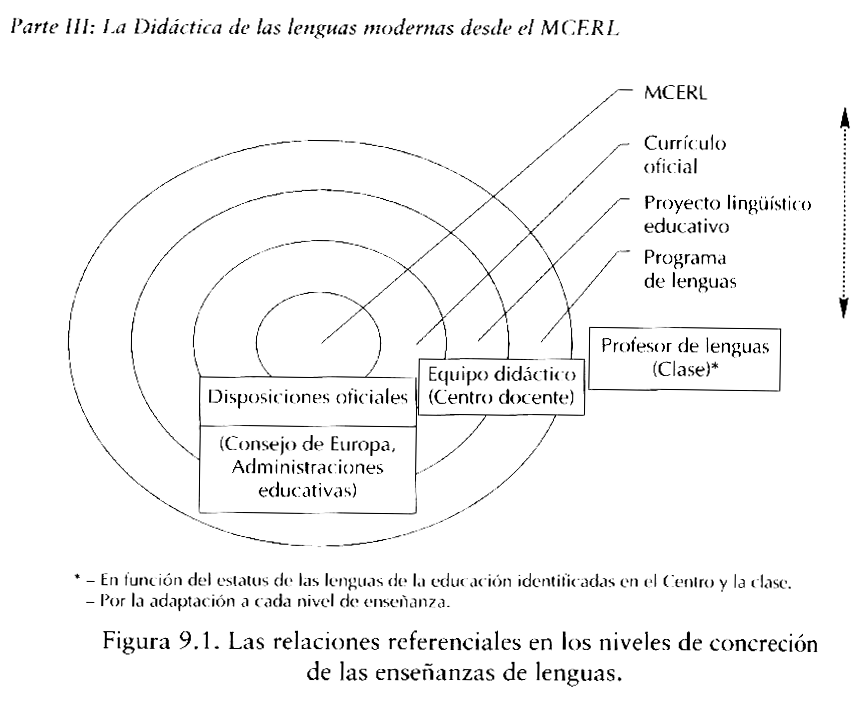
\includegraphics{assets/01_01-HD.png}

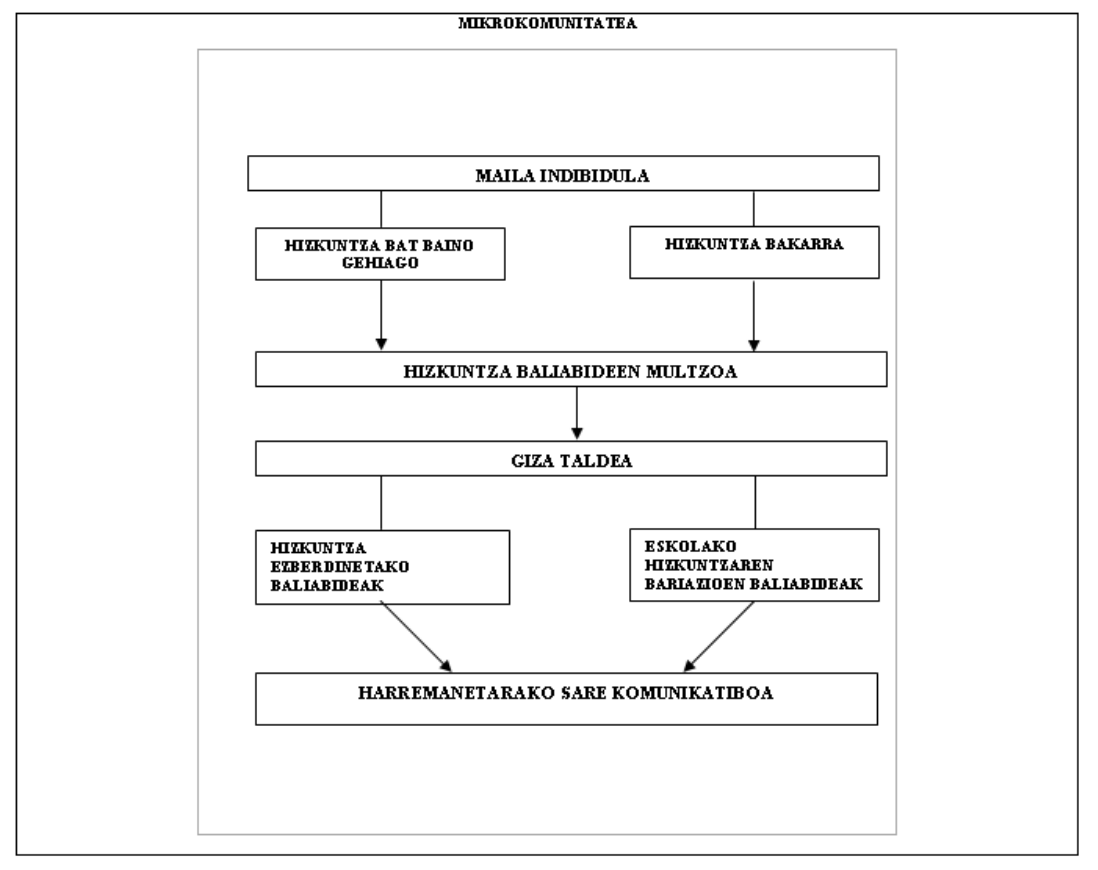
\includegraphics{assets/01_02-HD.png}

\hypertarget{metodoak}{%
\section{Metodoak}\label{metodoak}}

\textbf{Hizkuntza ulertzeko modua}-\textbf{Irakasteko modua}-\textbf{Metodologia ezberdinak}

\begin{itemize}
\tightlist
\item
  Gramatika/itzulpen metodoak
\item
  Eredu audiolinguala(egituren errepikapena, buruz ikasi)
\item
  Eredu kognoszitiboa (arauak)
\item
  Pragmatika eta eredu nozional/komunikaziozkoa:\emph{The communicative approach}
\end{itemize}

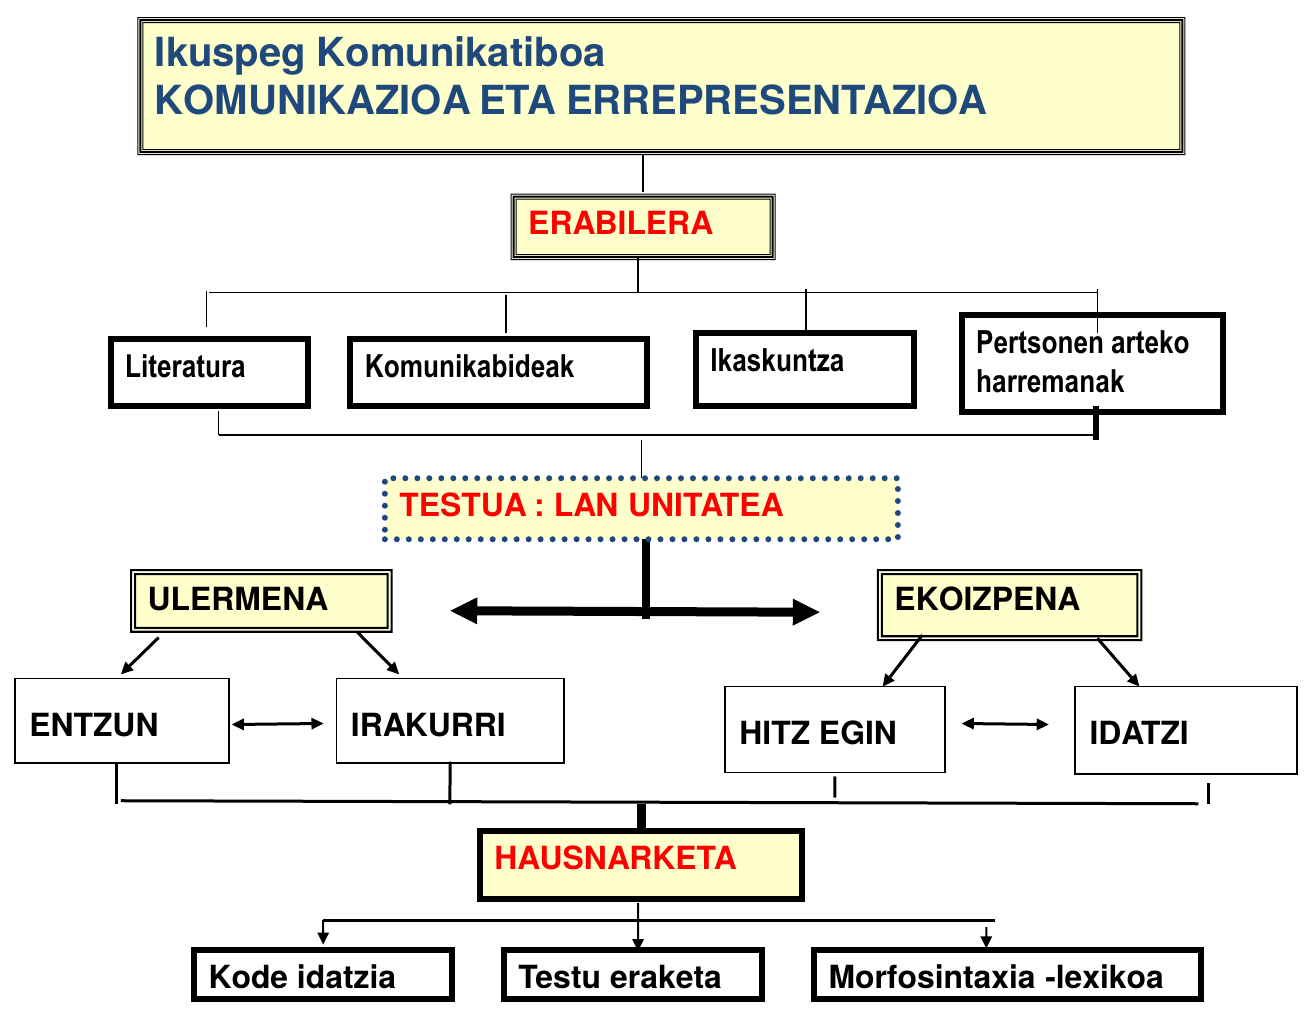
\includegraphics{assets/01_03-HD.png}

Testu horiek era egokian ``erabiltzea'' nahi badugu, gure lan eduki nagusiak trebezia mailakoak izango dira: hitz egiten, idazten, irakurtzen, entzuten irakastea izango da gure zeregina.
Eta testu horiek gero eta hobeto erabili ahal izateko, gero eta hobeto hitz egin, idatzi, irakurri edo entzuteko, egiten dugun horren inguruko hausnarketa beharko dugu. Gramatika eta hizkuntzaren sistemaren gaineko lanak beste era bateko funtzioa hartzen du, ez da aprendizaiaren helburu, baizik eta baliabide

\begin{center}\rule{0.5\linewidth}{\linethickness}\end{center}

\hypertarget{erreferentziak}{%
\section{Erreferentziak}\label{erreferentziak}}

Idiazabal I.(2003). Eskolaren kalitatea eta euskara.\emph{BAT Soziolinguistika Aldizkaria} 49, 2003, 195-199. ISSN: 1130-8435

Idiazabal, I., \& Manterola, I. (2009). Euskal eredu elebidunak, murgilketa eta hizkuntzen irakaskuntza bateratua: kontzeptuen berrikusketa. \emph{Euskera}, 54, 2--1. Eskuragarri \url{http://www.euskaltzaindia.net/dok/euskera/74632.pdf} helbidean

Lewis, M. P.(2005). Towards a categorization of endangerment of the world's languages.\_SIL International\_.

López Valero, A. (1998). Hacia una conformación histórica de la Didáctica de la Lengua y la Literatura. \emph{Didáctica. Lengua y literatura}, (10), 215--232.

Martí, F., Ortega, P., Idiazabal, I., Barreña, A., Juaristi, P., Junyent, C., \ldots{} Amorrortu, E.(2005).\emph{Hizkuntzen mundua. Munduko hizkuntzei buruzko txostena}. Bilbo: UPV/EHU.

Moreno-Cabrera, J. C.(2008).\_El nacionalismo lingüístico: Una ideología destructiva\_. Barcelona: Ediciones Península.

Sánchez, J. M.(1991). \emph{Un futuro para nuestro pasado. Claves de la recuperación del Euskara y teoría social de las lenguas} (Libk. 1). Donostia: Gipuzkoako Foru Aldundia. Berreskuratua \href{http://www.ehu.eus/ojs/index.php/ASJU/article/view/8593-\%28e\%29tik}{http://www.ehu.eus/ojs/index.php/ASJU/article/view/8593}-tik

\hypertarget{lehenengo-jarduera}{%
\chapter*{Lehenengo jarduera}\label{lehenengo-jarduera}}
\addcontentsline{toc}{chapter}{Lehenengo jarduera}

\begin{itemize}
\tightlist
\item
  {[} {]} Landu Idiazabal \& Manterola (2008) testua, bertako kontzeptu gakoak ulertze aldera.
\end{itemize}

\hypertarget{taldearen-hizkuntz-esperientzia}{%
\subsection{Taldearen hizkuntz esperientzia}\label{taldearen-hizkuntz-esperientzia}}

Ikaskideen aurreko aurkezpena egin behar duzue aipatu testuko gako idiak kontuan izanda.

\hypertarget{hautazko-jarduera}{%
\section{Hautazko jarduera:}\label{hautazko-jarduera}}

\begin{itemize}
\tightlist
\item
  {[} {]} Irakurri \emph{Txepetx}ek\footnote{\emph{Txepetx} da Jose Maria Sánchezen desizena. izenpetu ere bere desizenez egiten zuenez, hori ere erabiltzeko ohitura zabaldu da.} dioena eta erantzun galderak. Horretarako aparteko laburpena dago, Telegrameko kanaleko lehenengotariko dokumentua edo \href{https://github.com/JuanAbasolo/HD/blob/01-gaia/1_Txepetx_testuak.pdf}{esteka honetan}.
\end{itemize}

\hypertarget{ahozko-aurkezpena-ebaluatzeko-errubrika}{%
\chapter*{Ahozko aurkezpena ebaluatzeko errubrika}\label{ahozko-aurkezpena-ebaluatzeko-errubrika}}
\addcontentsline{toc}{chapter}{Ahozko aurkezpena ebaluatzeko errubrika}

Hurrengo errubrika hau erabiliko dugu ahozko ebaluazioetarako

\begin{longtable}[]{@{}rllll@{}}
\toprule
\begin{minipage}[b]{0.11\columnwidth}\raggedleft
\strut
\end{minipage} & \begin{minipage}[b]{0.19\columnwidth}\raggedright
\textbf{Hobekuntza franko behar duen lana}\strut
\end{minipage} & \begin{minipage}[b]{0.19\columnwidth}\raggedright
\textbf{Lan nahikoa}\strut
\end{minipage} & \begin{minipage}[b]{0.19\columnwidth}\raggedright
\textbf{Lan ona}\strut
\end{minipage} & \begin{minipage}[b]{0.19\columnwidth}\raggedright
\textbf{Lan bikaina}\strut
\end{minipage}\tabularnewline
\midrule
\endhead
\begin{minipage}[t]{0.11\columnwidth}\raggedleft
\textbf{Taldeko lana}\strut
\end{minipage} & \begin{minipage}[t]{0.19\columnwidth}\raggedright
Taldekideen artean ez da elkarlanik egon eta lanean nabaritzen da\strut
\end{minipage} & \begin{minipage}[t]{0.19\columnwidth}\raggedright
Kohesio falta dago, lana taldekideen artean banatu dute baina oso zaila da tokatu zaien zatiaz hitz egitea.\strut
\end{minipage} & \begin{minipage}[t]{0.19\columnwidth}\raggedright
Lana taldekideen artean banatu dute baina azken entsegua denen artean egin dute.\strut
\end{minipage} & \begin{minipage}[t]{0.19\columnwidth}\raggedright
Koordinazio eta komunikazio handia dago, guztiek tokatu zaien zatia ondo egin dute.\strut
\end{minipage}\tabularnewline
\begin{minipage}[t]{0.11\columnwidth}\raggedleft
\textbf{Edukiak}\strut
\end{minipage} & \begin{minipage}[t]{0.19\columnwidth}\raggedright
Edukiak txarto hautau dituzte, txarto antolatuta daude eta errepikatuta\strut
\end{minipage} & \begin{minipage}[t]{0.19\columnwidth}\raggedright
Edukiak egokiak dira, baina edukiak hobeto antolatu daitezke\strut
\end{minipage} & \begin{minipage}[t]{0.19\columnwidth}\raggedright
Edukiak ondo aukeratu dituzte, ondo antolatuta daude eta ondo azalduta\strut
\end{minipage} & \begin{minipage}[t]{0.19\columnwidth}\raggedright
Edukiak ondo aukeratu dituzte, ondo antolatuta daude eta ondo azalduta.\strut
\end{minipage}\tabularnewline
\begin{minipage}[t]{0.11\columnwidth}\raggedleft
\textbf{Irudia}\strut
\end{minipage} & \begin{minipage}[t]{0.19\columnwidth}\raggedright
Kolorea txarto aukeratu da, testu gehiegi, ikusteko arazoak.\strut
\end{minipage} & \begin{minipage}[t]{0.19\columnwidth}\raggedright
Aurkezpena ondo ikusten da, baina itxusia da.\strut
\end{minipage} & \begin{minipage}[t]{0.19\columnwidth}\raggedright
Argazkiak ondo aukeratu dira, testua orekatua da, ondo ikusten da.\strut
\end{minipage} & \begin{minipage}[t]{0.19\columnwidth}\raggedright
Argazkiak ondo aukeratu dira, testua orekatua da, gainera, ikusten dena oso erakargarria da.\strut
\end{minipage}\tabularnewline
\begin{minipage}[t]{0.11\columnwidth}\raggedleft
\textbf{Ahozko aurkezpena}\strut
\end{minipage} & \begin{minipage}[t]{0.19\columnwidth}\raggedright
Isilune handiak, testua falta da. Diapositibak nahasten dira.\strut
\end{minipage} & \begin{minipage}[t]{0.19\columnwidth}\raggedright
Aurkezpena egokia da, baina denboretara egokitzeko arazoak. Ahozkera arazoak.\strut
\end{minipage} & \begin{minipage}[t]{0.19\columnwidth}\raggedright
Aurkezpen egokia, denboretara ondo egokituta, ahozkera ona.\strut
\end{minipage} & \begin{minipage}[t]{0.19\columnwidth}\raggedright
Aurkezpen egokia, denboretara ondo egokituta, ahozkera ona. Gorpuzkerak, aurpegikerak eta keinuek diskurtsoari indarra ematen diote.\strut
\end{minipage}\tabularnewline
\bottomrule
\end{longtable}

\hypertarget{hizkuntza-eta-ageriko-curriculuma}{%
\chapter{Hizkuntza eta ageriko curriculuma}\label{hizkuntza-eta-ageriko-curriculuma}}

\href{https://gitpitch.com/JuanAbasolo/HD/02-gaia?grs=github\&t=moon}{
\includegraphics{assets/badge.png}}

Hizkuntza eskolan tratatzeko erez ari garenean, kontuan izan behar dugu horren inguruan ereikitako lege ikuspegi osoa. Besteak beste, horren arabera sortu beharko duzuelako dena delako elementua oposizioak-eta egiteko.

Curriculumez ari garenean hitz egin dezakegu eskola esperientziak eragindako bizipen/ikaskuntzez edota aurrez prestatutako ikaskuntza-ibilbiderako planez. Oraingo honetan bigarren horri buruz hausnartu behar dugu: Curriculum diseinuaz.

Legeen bitartez eraikitzen da curriculumaren lehenengo zehaztapen maila. Kapitulu honetan legeei begiratu behar diegu, zehazki, hizkuntzari begiratzen dion alderdia landuko dugu.

Lege markoa matroysken antzera eregiten da, pausu bakoitzak jarraikortasuna behar du aurrekoarekiko. Euskal Herriko ikasgeletara iristen den legearen forma aurretiko beste lege batzuk moldatutakoa da.

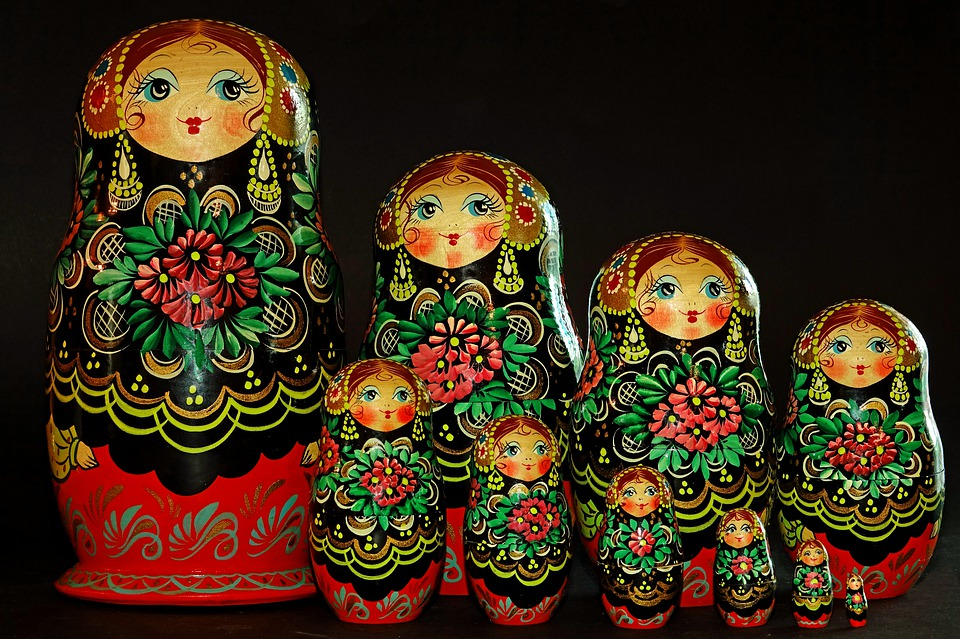
\includegraphics{assets/ornament-3131097_960_720.jpg}
\href{https://pixabay.com/en/ornament-matryoshka-babuschka-3131097/}{iturria}

Gure kasuan, UPV/EHUk baskongadetako errealitateari begiratu behar dionez, Heziberri 2020 planak ezartzen duen errealitatea aztertuko dugu. Baina Euskal Herriko ikuspegi zabalago batetik ere begira genezaioke Ipar Euskal Herriko lege markoa edota Nafarroakora egokituta, dagozkien elementuak.

Gaur egungo paradigmatik ulertuta, hezkuntzaz aritzeak esan nahi du gaikuntzaz hitz egitea, gaitasunak garatzeari buruz jardutea.

Horrela, gaurko lege-markoa ulertzeko paradigamren eraikuntzatik hasi, legeek egiten duten interpretaziora pasa eta gelako jardunaren diseinura iritsi behar dugu. Matryoskak bailiran legez

\begin{itemize}
\tightlist
\item
  Delors txostena (UNESCO) 1998\\
  Education for the twenty-first century: issues and prospects: contributions to the work of the International Commission on Education for the Twenty-First Century (\href{http://unesdoc.unesco.org/images/0011/001147/114766e.pdf}{en})\\
  La educación encierra un tesoro (\href{http://www.unesco.org/education/pdf/DELORS_S.PDF}{es})
\item
  DeSeCo (OCDE)
  Definition and Selection of Competences (DeSeCo): Theoretical and conceptual foundations (2002)\href{http://deseco.ch/bfs/deseco/en/index/02.parsys.34116.downloadList.87902.DownloadFile.tmp/oecddesecostrategypaperdeelsaedcericd20029.pdf}{(*)}
  Key Competencies for a Successful Life and a Well-Functioning Society (2003)
  Definition and Selection of Key Competencies - Executive Summary\href{http://deseco.ch/bfs/deseco/en/index/02.parsys.43469.downloadList.2296.DownloadFile.tmp/2005.dskcexecutivesummary.en.pdf}{*} (2005)
\item
  Gaitasun giltzarriak (Europar Legebiltzarra)
  \href{http://eur-lex.europa.eu/legal-content/EN/TXT/?uri=CELEX:32006H0962}{2006/962/CE} (\href{http://infofpe.cea.es/fpe/norm/Rec\%2018_2006.pdf}{es})
  Recommendation of the European Parliament and of the Council of 18 December 2006 on key competences for lifelong learning.
\item
  LOMCE 8/2013 + Frantziako ordenamendua
\item
  Curriculuma 126/2014 + Frantziako Curriculuma
\item
  Agindua ECD/65/2015 + Frantziako baliokidea
\item
  Oinarrizko Hezkuntzarako curriculum Dekretua + Nafarroako ordenamendua
\end{itemize}

\begin{center}\rule{0.5\linewidth}{\linethickness}\end{center}

\hypertarget{hegoaldeko-lege-markoa}{%
\section{Hegoaldeko lege markoa}\label{hegoaldeko-lege-markoa}}

Hemen Hegoaldeko kasuaren azterketan ardazten ari gara analisia, baina berdin egin liteke Iparraldeari begiratu nahi bageuntse Frantziako kasua aztertuaz. Hori ikusteko, \href{http://www.vc.ehu.es/araka/orri12.htm}{Araka}ko web orriko baliabideak interesgarriak izan daitezke, baina kontuan izan behar da azken legeak ez dituela hartzen.

\hypertarget{lomce}{%
\subsection{LOMCE}\label{lomce}}

Ley Orgánica 8/2013, de 9 de diciembre, para la mejora de la calidad educativa\href{https://www.boe.es/buscar/act.php?id=BOE-A-2013-12886}{*}.

\begin{quote}
\ldots{} Obligatoria en un curso fundamentalmente propedéutico y con dos trayectorias bien diferenciadas.

La LOMCE hace especial incidencia con vistas a la transformación del sistema educativo: las Tecnologías de la Información y la Comunicación, el fomento del plurilingüismo, y la modernización de la Formación Profesional.
\end{quote}

\hypertarget{curriculuma-ezartzeko-dekretua}{%
\subsection{Curriculuma ezartzeko dekretua}\label{curriculuma-ezartzeko-dekretua}}

126/2014 Erret dekretua\href{https://www.boe.es/buscar/pdf/2014/BOE-A-2014-2222-consolidado.pdf}{*}

Real Decreto 126/2014, de 28 de febrero, por el que se establece el currículo básico de la Educación Primaria\href{https://www.boe.es/buscar/pdf/2014/BOE-A-2014-2222-consolidado.pdf}{*}.

\begin{quote}
\ldots{}se entiende por currículo la regulación de los elementos que determinan los procesos de enseñanza y aprendizaje para cada una de las enseñanzas\ldots{}
\end{quote}

Ikasgaien antolaketa ere dekretu horretan zehazten da:

\begin{itemize}
\tightlist
\item
  Curriculuma
\item
  Helburuak
\item
  Konpetentziak
\item
  Edukiak
\item
  Ikaskuntza estandarrak
\item
  Ebaluazio irizpideak
\item
  Metodologia didaktikoa
\end{itemize}

\hypertarget{gaitasunak-edukiak-eta-ebaluazio-irizpideak}{%
\subsection{Gaitasunak, edukiak eta ebaluazio irizpideak}\label{gaitasunak-edukiak-eta-ebaluazio-irizpideak}}

Zehazten dira ECD/65/2015 Aginduan\href{https://www.boe.es/buscar/doc.php?id=BOE-A-2015-738}{*}

Orden ECD/65/2015, de 21 de enero, por la que se describen las relaciones entre las competencias, los contenidos y los criterios de evaluación de la educación primaria, la educación secundaria obligatoria y el bachillerato

\hypertarget{honako-konpetentziak-zehazten-dira}{%
\subsubsection{Honako konpetentziak zehazten dira:}\label{honako-konpetentziak-zehazten-dira}}

\begin{enumerate}
\def\labelenumi{\arabic{enumi}.}
\tightlist
\item
  Comunicación lingüística.
\item
  Competencia matemática y competencias básicas en ciencia y tecnología.
\item
  Competencia digital.
\item
  Aprender a aprender.
\item
  Competencias sociales y cívicas.
\item
  Sentido de iniciativa y espíritu emprendedor.
\item
  Conciencia y expresiones culturales.
\end{enumerate}

\hypertarget{legedia-hizkuntzaren-didaktikaren-arautzailea}{%
\subsection{Legedia, hizkuntzaren didaktikaren arautzailea}\label{legedia-hizkuntzaren-didaktikaren-arautzailea}}

\begin{longtable}[]{@{}rccccc@{}}
\toprule
\begin{minipage}[b]{0.11\columnwidth}\raggedleft
\strut
\end{minipage} & \begin{minipage}[b]{0.14\columnwidth}\centering
Ebaluazioa\strut
\end{minipage} & \begin{minipage}[b]{0.14\columnwidth}\centering
Hizkuntza ofizial eta koofizialak\strut
\end{minipage} & \begin{minipage}[b]{0.14\columnwidth}\centering
Atzerriko hizkuntza\strut
\end{minipage} & \begin{minipage}[b]{0.14\columnwidth}\centering
Komunikazio gaitasuna\strut
\end{minipage} & \begin{minipage}[b]{0.14\columnwidth}\centering
Ikuspuntu komunikatiboa\strut
\end{minipage}\tabularnewline
\midrule
\endhead
\begin{minipage}[t]{0.11\columnwidth}\raggedleft
\textbf{LOMCE}\strut
\end{minipage} & \begin{minipage}[t]{0.14\columnwidth}\centering
x\strut
\end{minipage} & \begin{minipage}[t]{0.14\columnwidth}\centering
\strut
\end{minipage} & \begin{minipage}[t]{0.14\columnwidth}\centering
\strut
\end{minipage} & \begin{minipage}[t]{0.14\columnwidth}\centering
\strut
\end{minipage} & \begin{minipage}[t]{0.14\columnwidth}\centering
\strut
\end{minipage}\tabularnewline
\begin{minipage}[t]{0.11\columnwidth}\raggedleft
\textbf{Curriculum Dekretua}\strut
\end{minipage} & \begin{minipage}[t]{0.14\columnwidth}\centering
x\strut
\end{minipage} & \begin{minipage}[t]{0.14\columnwidth}\centering
x\strut
\end{minipage} & \begin{minipage}[t]{0.14\columnwidth}\centering
x\strut
\end{minipage} & \begin{minipage}[t]{0.14\columnwidth}\centering
x\strut
\end{minipage} & \begin{minipage}[t]{0.14\columnwidth}\centering
\strut
\end{minipage}\tabularnewline
\begin{minipage}[t]{0.11\columnwidth}\raggedleft
\textbf{ECD 65/2015 Agindua}\strut
\end{minipage} & \begin{minipage}[t]{0.14\columnwidth}\centering
\strut
\end{minipage} & \begin{minipage}[t]{0.14\columnwidth}\centering
\strut
\end{minipage} & \begin{minipage}[t]{0.14\columnwidth}\centering
\strut
\end{minipage} & \begin{minipage}[t]{0.14\columnwidth}\centering
x\strut
\end{minipage} & \begin{minipage}[t]{0.14\columnwidth}\centering
\strut
\end{minipage}\tabularnewline
\begin{minipage}[t]{0.11\columnwidth}\raggedleft
\textbf{Heziberri 2020}\strut
\end{minipage} & \begin{minipage}[t]{0.14\columnwidth}\centering
x\strut
\end{minipage} & \begin{minipage}[t]{0.14\columnwidth}\centering
x\strut
\end{minipage} & \begin{minipage}[t]{0.14\columnwidth}\centering
x\strut
\end{minipage} & \begin{minipage}[t]{0.14\columnwidth}\centering
x\strut
\end{minipage} & \begin{minipage}[t]{0.14\columnwidth}\centering
x\strut
\end{minipage}\tabularnewline
\bottomrule
\end{longtable}

\hypertarget{oinarrizko-konpetentzia-giltzei-buruzko-proposamen-arteko-erlazioa}{%
\section{\texorpdfstring{Oinarrizko konpetentzia giltzei buruzko proposamen arteko erlazioa \href{http://www.hezkuntza.ejgv.euskadi.eus/contenidos/informacion/heziberri_2020/eu_erlazioa/adjuntos/oinarrizko_konpetentzia_giltzei_buruzko_proposamen_arteko_erlazioa.pdf}{*}}{Oinarrizko konpetentzia giltzei buruzko proposamen arteko erlazioa *}}\label{oinarrizko-konpetentzia-giltzei-buruzko-proposamen-arteko-erlazioa}}

\begin{figure}
\centering
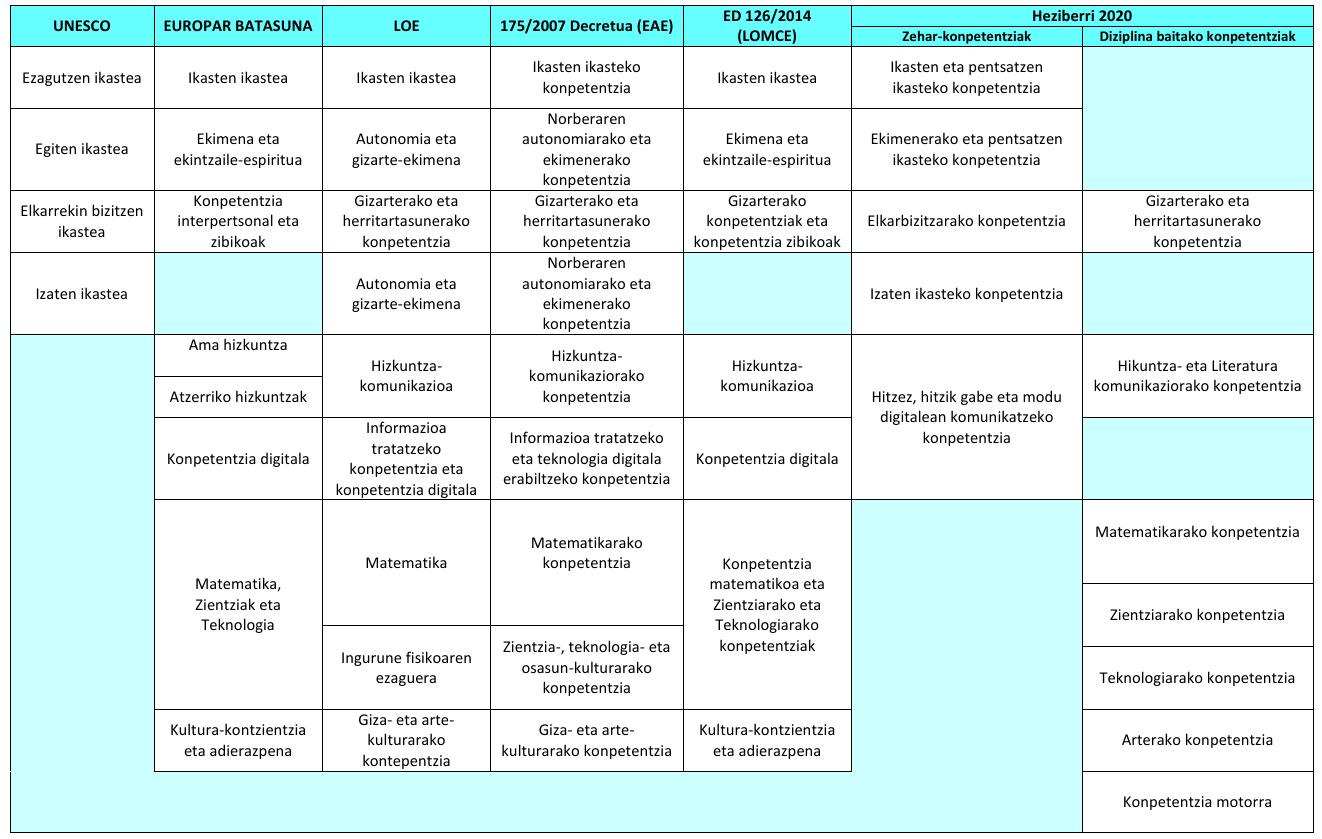
\includegraphics{assets/02_01-HD.png}
\caption{EJ}
\end{figure}

\hypertarget{baskongadeei-dagokien-araudia}{%
\section{Baskongadeei dagokien araudia}\label{baskongadeei-dagokien-araudia}}

Kontuan izan dezagun, soilik Euskal Autonomia Elkarteaz ari bagara, ez dugula kontuan hartzen Hegoaldeko hezkuntza errealitatea. Ber analisia egin dakioke Nafar curriculumari zein besteren bati ere.

\hypertarget{oinarrizko-hezkuntzarako-curriculum-dekretua}{%
\subsection{\texorpdfstring{Oinarrizko Hezkuntzarako curriculum dekretua \href{https://www.euskadi.eus/y22-bopv/eu/bopv2/datos/2016/01/1600141e.shtml}{*}}{Oinarrizko Hezkuntzarako curriculum dekretua *}}\label{oinarrizko-hezkuntzarako-curriculum-dekretua}}

\href{http://www.jusap.ejgv.euskadi.eus/r47-bopvapps/es/bopv2/datos/2016/01/1600141e.pdf}{236/2015 Dekretua}, abenduaren 22koa, Oinarrizko Hezkuntzaren curriculuma zehaztu eta Euskal Autonomia Erkidegoan ezartzen duena (EHAA, 2016-01-15)

\hypertarget{hizkuntza--eta-literatura--komunikaziorako-konpetentzia.}{%
\subsubsection{1. Hizkuntza- eta literatura- komunikaziorako konpetentzia.}\label{hizkuntza--eta-literatura--komunikaziorako-konpetentzia.}}

1.1.2.-- Eduki multzoen ezaugarriak.

Lehen Hezkuntzari dagozkion adierazpenezko, prozedurazko eta jarrerazko edukiak honako eduki multzo hauetan multzokatzen dira:

\hypertarget{eduki-multzoak}{%
\subsubsection{Eduki multzoak}\label{eduki-multzoak}}

\begin{enumerate}
\def\labelenumi{\arabic{enumi}.}
\tightlist
\item
  Arlo guztietan komunak diren oinarrizko zehar-konpetentziekin lotutako edukiak.
\item
  Ahozko komunikazioa: hitz egitea, entzutea eta elkarrekin solasean jardutea.
\item
  Idatzizko komunikazioa: irakurtzea eta idaztea.
\item
  Literatura-hezkuntza.
\item
  Hizkuntzari eta haren erabilerei buruzko gogoeta.
\item
  Hizkuntzaren alderdi soziala.
\end{enumerate}

\begin{center}\rule{0.5\linewidth}{\linethickness}\end{center}

\hypertarget{kapituluko-erreferentziak}{%
\section{Kapituluko erreferentziak}\label{kapituluko-erreferentziak}}

Araka ikertaldea. (2003). Araka ikertaldea - legeria \[web\]. Berreskuratua 2018(e)ko otsailakaren 9a, \url{http://www.vc.ehu.es/araka/orri12.htm} etik

Centro Universitario de Desarrollo Intelectual. (2016). Catálogo de rúbricas para la evaluación del aprendizaje. Berreskuratua \href{http://evirtual.uaslp.mx/FCQ/estrategias/Material\%20de\%20Apoyo/cat_rubrica.pdf}{http://evirtual.uaslp.mx/FCQ/estrategias/Material de Apoyo/cat\_rubrica.pdf} -etik

Delors, J., International Commission on Education for the Twenty-First Century, \& UNESCO (Arg.). (1998). \emph{Education for the twenty-first century: issues and prospects: contributions to the work of the International Commission on Education for the Twenty-First Century}. Paris: UNESCO Publishing.

EURIDYCE (Arg.). (2002). \emph{Key competencies: a developing concept in general compulsory education}. Brussels.

Europar Batasuna. (2006). \emph{2006/962/CE Recommendation of the European Parliament and of the Council of 18 December 2006 on key competences for lifelong learning} (Gomendioa No.~32006H0962) (or. 10\textasciitilde{}18). Estrasburgo: Europako Parlamentua. Berreskuratua \url{http://data.europa.eu/eli/reco/2006/962/oj/eng} -etik

EURYDICE. (2003). \emph{Las Competencias clave: un concepto en expansión dentro de la educación general obligatoria.} Madril: Eurydice. Unidad Española. Berreskuratua \url{http://www.hezkuntza.ejgv.euskadi.eus/contenidos/informacion/dig_publicaciones_innovacion/es_curricul/adjuntos/14_curriculum_competencias_300/300001c_Pub_UE_Eurydice_Competencias_c.pdf} -etik

Eusko Jaurlaritza (Hezkuntza, Hizkuntza Politika eta Kultura Saila). (2017). Oinarrizko konpetentzia giltzei buruzko proposamen arteko erlazioa \[pdf formatudun dokumentoa\]. Berreskuratua 2018(e)ko otsailakaren 9a, \url{http://www.hezkuntza.ejgv.euskadi.eus/contenidos/informacion/heziberri_2020/eu_erlazioa/adjuntos/oinarrizko_konpetentzia_giltzei_buruzko_proposamen_arteko_erlazioa.pdf} -etik

Eusko Jaurlaritzaren legebiltzarra. (2015). 236/2015 Dekretua, abenduaren 22koa, Oinarrizko Hezkuntzaren curriculuma zehaztu eta Euskal Autonomia Erkidegoan ezartzen duena. \emph{Euskal Herriko Agintaritzaren Aldizkaria, 2016ko urtarrilaren 15a}, \emph{141}. Berreskuratua \url{https://www.euskadi.eus/y22-bopv/eu/bopv2/datos/2016/01/1600141e.shtml} -etik

Gobierno de España. (2013). Ley Orgánica 8/2013, de 9 de diciembre, para la mejora de la calidad educativa. \emph{Boletín Oficial del Estado}. Berreskuratua \url{https://www.boe.es/buscar/act.php?id=BOE-A-2013-12886} -tik

Gobierno de España (Ministerio de Educación, Cultura y Deporte). (2014). Real Decreto 126/2014, de 28 de febrero, por el que se establece el currículo básico de la Educación Primaria. \emph{Boletín Oficial del Estado}, \emph{52}, 19349--19420. Berresekuratua \url{https://www.boe.es/buscar/act.php?id=BOE-A-2014-2222} -tik

Gobierno de España (Ministerio de Educación, Cultura y Deporte). (2015). Orden Ecd/65/2015, de 21 de enero, por la que se describen las relaciones entre las competencias, los contenidos y los criterios de evaluación de la educación primaria, la educación secundaria obligatoria y el bachillerato. \emph{Boletín Oficial de Estado}, (25). Berreskuratua \url{https://www.boe.es/buscar/doc.php?id=BOE-A-2015-738} -tik

Organisation for Economic Co-operation and Development. (2002, urriak 7). Definition and Selection of Competences (DeSeCo): Theoretical and conceptual foundations. Berreskuratua \url{http://deseco.ch/bfs/deseco/en/index/02.parsys.34116.downloadList.87902.DownloadFile.tmp/oecddesecostrategypaperdeelsaedcericd20029.pdf} -etik

Organisation for Economic Co-operation, \& Development (OECD). (2005). \emph{The definition and selection of key competencies: Executive summary}. OECD Paris. Berreskuratua \url{http://deseco.ch/bfs/deseco/en/index/02.html} -etik

Organización para la Cooperación y el Desarrollo Económicos (OCDE). (2015). \emph{La definición selección de las competencias clave. Resumen ejecutivo}.

Rychen, D. S., \& Salganik, L. H. (Arg.). (2003). \emph{Key competencies for a successful life and a well-functioning society}. Cambridge, Massachusetts: Hogrefe \& Huber.

\hypertarget{bigarren-jarduera}{%
\chapter*{Bigarren jarduera}\label{bigarren-jarduera}}
\addcontentsline{toc}{chapter}{Bigarren jarduera}

\begin{itemize}
\item
  Oinarrizko Hezkuntzako Curriculuma
  (236/2015eko Dekretuaren II. Eranskina osatzen duen curriculum orientatzailea)
\item
  Aurkeztu eta konpartitu:
  Sort ezazu egokitu zaizuen multzoaren eskema. Ikaskideei aurkeztu eta eurekin partekatu beharko duzue.
\end{itemize}

\textbf{Ebaluazioa} egiteko \href{http://evirtual.uaslp.mx/FCQ/estrategias/Material\%20de\%20Apoyo/cat_rubrica.pdf}{hau} erabiliko dut.

\hypertarget{ahozko-trebetasuna-lhn}{%
\chapter{Ahozko Trebetasuna LHn}\label{ahozko-trebetasuna-lhn}}

\href{../Diapoak/03_Diap-ahozko_trebetasunak.html}{
\includegraphics{assets/badge.png}}

Hizkuntzen irakaskuntzan ikuspegi eta metodo ezberdinak eraman dira
praktikara eta ahozko komunikazioak ez du beti toki bera izan:

\begin{longtable}[]{@{}lll@{}}
\caption{Metodoen garapenaz}\tabularnewline
\toprule
\begin{minipage}[b]{0.21\columnwidth}\raggedright
\strut
\end{minipage} & \begin{minipage}[b]{0.35\columnwidth}\raggedright
Ikuspegia/Metodoa\strut
\end{minipage} & \begin{minipage}[b]{0.35\columnwidth}\raggedright
Ahozkotasunarenirakaskuntza\strut
\end{minipage}\tabularnewline
\midrule
\endfirsthead
\toprule
\begin{minipage}[b]{0.21\columnwidth}\raggedright
\strut
\end{minipage} & \begin{minipage}[b]{0.35\columnwidth}\raggedright
Ikuspegia/Metodoa\strut
\end{minipage} & \begin{minipage}[b]{0.35\columnwidth}\raggedright
Ahozkotasunarenirakaskuntza\strut
\end{minipage}\tabularnewline
\midrule
\endhead
\begin{minipage}[t]{0.21\columnwidth}\raggedright
XX. Mendearen aurretik\strut
\end{minipage} & \begin{minipage}[t]{0.35\columnwidth}\raggedright
Metodo zuzena edo Naturala\strut
\end{minipage} & \begin{minipage}[t]{0.35\columnwidth}\raggedright
Ahozko elkarreragina:irakaslearen galdera-ikaslearen erantzuna\strut
\end{minipage}\tabularnewline
\begin{minipage}[t]{0.21\columnwidth}\raggedright
XX. mendea\strut
\end{minipage} & \begin{minipage}[t]{0.35\columnwidth}\raggedright
Metodo Estrukturalistak:Situaliazionala eta Audiolinguala\strut
\end{minipage} & \begin{minipage}[t]{0.35\columnwidth}\raggedright
Egituren errepikapenaDena ahoz lantzen da eta idatzizko hizkuntza bigarren maila\strut
\end{minipage}\tabularnewline
\begin{minipage}[t]{0.21\columnwidth}\raggedright
Ikuspegi eta metodo alternatiboak\strut
\end{minipage} & \begin{minipage}[t]{0.35\columnwidth}\raggedright
Erantzun fisiko Totala, Metodo Isila,Hizkuntzaren Ikaskuntza Komunitarioa,Sugestopedia,Adimen anitzak,Ikuspegi Lexikoaeta Gaitasunetan Oinarritutako Hizkuntzen Irakaskuntza.\strut
\end{minipage} & \begin{minipage}[t]{0.35\columnwidth}\raggedright
Gramatikaren irakaspenari emandako garrantzitik alde egin nahi zuten, eta ikasgeletan elkarrizketarako tartea zabaldu.\strut
\end{minipage}\tabularnewline
\begin{minipage}[t]{0.21\columnwidth}\raggedright
Gaur egungo ikuspegi komunikatiboak\strut
\end{minipage} & \begin{minipage}[t]{0.35\columnwidth}\raggedright
Hizkuntzaren Irakaskuntza Komunikatiboa,Ikuspegi Naturala,Hizkuntzaren Ikaskuntza Kooperatiboa,Edukietan Oinarritutako Instrukzioa,Atazetan Oinarritutako Hizkuntzaren Irakaskuntza eta post-metodo aroa.\strut
\end{minipage} & \begin{minipage}[t]{0.35\columnwidth}\raggedright
Ikasleen arteko harremanak sortzea; ez bakarrik egiturak ezagutzea.Ikasleek hizkuntza ikasiko dute komunikatzeko beharragatik\strut
\end{minipage}\tabularnewline
\bottomrule
\end{longtable}

\hypertarget{ahozko-ekoizpen-eta-jarduera-motak}{%
\section{Ahozko ekoizpen eta jarduera motak}\label{ahozko-ekoizpen-eta-jarduera-motak}}

\begin{itemize}
\tightlist
\item
  Adierazpen publikoak egitea (informazioa, jarraibideak, etab.)
\item
  Jendaurrean hitz egitea (azalpenak ematea bileretan, unibertsitateko hitzaldiak, sermoiak, ikuskizunak, kiroletako azalpenak, salmenten aurkezpenak, etab.)
\item
  Elkarrizketak
\end{itemize}

\ldots{}eta ekintza horiek hurrengoak eska ditzakete:

\begin{itemize}
\tightlist
\item
  Idatzizko testu bat ozen irakurtzea;
\item
  Oharretan, idatzizko testu batean edo ikusizko elementuetan (eskemak, irudiak,
  grafikoak, etab.) oinarrituta hitz egitea;
\item
  Aldez aurretik prestatutako zerbait antzeztea;
\item
  Bat-batean hitz egitea;
\item
  Abestea.
\end{itemize}

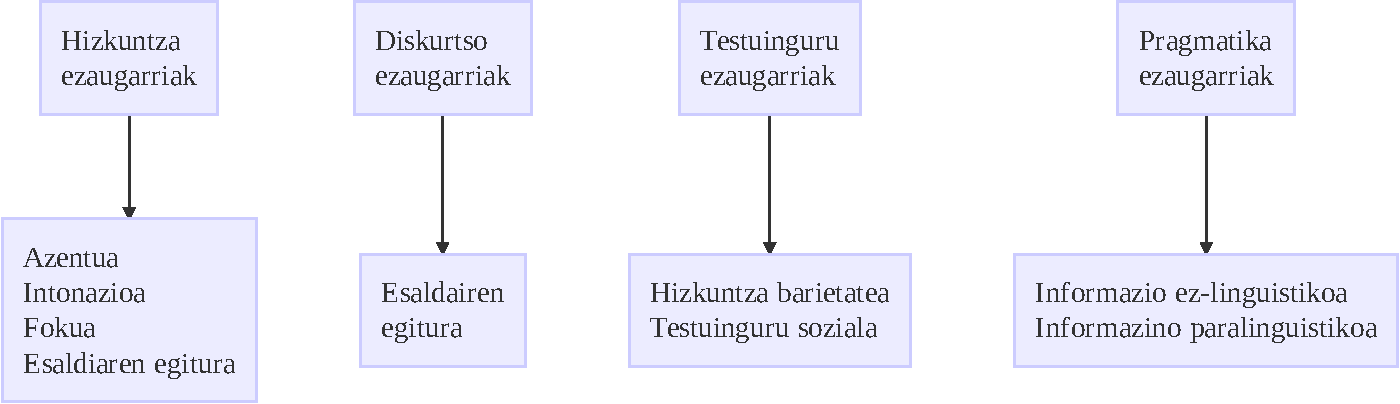
\includegraphics{bookdown-demo_files/figure-latex/unnamed-chunk-1-1.pdf}

\hypertarget{bazter-utzitako-eremua}{%
\section{Bazter utzitako eremua}\label{bazter-utzitako-eremua}}

\begin{quote}
Hizkuntzaren ikaskuntzan nahiz irakaskuntzan, sarritan, ahozkotasuna ahaztu
egin da. Horren ondorioz, ahozkotasunaren ezaugarri segmentalak
(kontsonanteak eta bokalak) nahiz suprasegmentalak (erritmoa, azentua eta
intonazioa) sarritan ez omen ditugu irakatsi

---\emph{Usó, 2008}
\end{quote}

\begin{quote}
El papel marginal de la pronunciación tanto en
los materiales didácticos (en la introducción, en
el apéndice, en actividades desligadas del tema
de la unidad\ldots{} ) como en las publicaciones en
el ámbito de la didáctica de la LE.

---\emph{Cortés Moreno, 2001: 128}
\end{quote}

\hypertarget{garrantziaz}{%
\subsection{Garrantziaz}\label{garrantziaz}}

\begin{quote}
Hoy en día, muchos profesionales sin conocimientos específicos de fonética
quieren o necesitan por motivos laborales adaptar su pronunciación al uso
estándar de la lengua y alejar, en su proyección pública, rasgos considerados
demasiado dialectales o marcados especialmente de algún modo. Pueden estar
en este caso periodistas, locutores de televisión y de radio, cantantes de éxito,
políticos, empresarios, financieros\ldots{} Para dirigirse a un amplio público y
transmitir mensajes alejados de la broma como puede ser un telediario o un
discurso de política general puede ser interesante intentar circunscribirse a un
estilo estándar formal de pronunciación para que aspectos marcadamente
dialectales o sociales no desvíen la atención del contenido que se pretende
transmitir. También puede verse en esta situación un actor o una actriz que para
poder trabajar deba disimular su acento original o, por el contrario, deba
adoptar un acento que no es el suyo nativo.

---\emph{Fernández, 2007:43}
\end{quote}

\hypertarget{baliabideak}{%
\subsection{Baliabideak}\label{baliabideak}}

BIDEOJOKOAK: Bideojokoak sortu izan dira behar bereziak dituztenei
laguntzeko (Corrales, 2015; Aguilar et. al., 2015), izan ere bideojokoek aukera
ematen dute errealiatea errepresentatzeko, hiztunen arteko erlazioak
adierazteko eta komunikazio egoeretan gertatzen diren kausa-ondorio erlazioak
lantzeko (Aguilar et. al., 2015).

\hypertarget{pradia-bideojokoa}{%
\subsubsection{\texorpdfstring{\href{http://pradia.net/}{Pradia} bideojokoa:}{Pradia bideojokoa:}}\label{pradia-bideojokoa}}

Intonazio eta emozio patroiak
Identifikatu eta lantzeko.
Batez ere behar bereziak dituzten
Umeentzako baliabidea da.

\hypertarget{jolasak}{%
\subsubsection{Jolasak}\label{jolasak}}

Hurrengoa Gaminde eta beste (2014) liburutik hartutako adibidea duzu

\begin{quote}
\textbf{ESKU JOLASA}

\textbf{Antolaketa}: Binaka.

\textbf{Helburua}: Emozioen adierazpena lantzea.

\textbf{Materiala}: Errezitatu bat.

\textbf{Prozesua}: Jolasarekin hasi aurretik: Irakasleak binaka jarriko ditu umeak
eta errezitatu bitartean zati batzuk pozik, haserre eta triste adieraziko
dituztela esango die, irakasleak aukeratuko du zer zati esango duten
pozik, haserre ala triste, eta emozio mota adierazten dutenean, ikasleek
era horretan errezitatuko dute.
Jolasaren hasieran: Errezitatu hau denen artean esango dute ahoz
gora:

\emph{Arre arre mandako\\
Bihar Tolosarako\\
Etzi Iruñerako\\
Handik zer ekarriko\\
Zapata ta gerriko}\\
---Gaminde, 2007

\emph{Jolastu bitartean}: Eskuekin binaka jolastuko dira, errezitatu bitartean
binaka ezkuekin jolastuko dira eta irakasleak emozio mota adieraztean
errezitatua adierazteko era emozio horretarako moldatuko dute.

---\emph{Gaminde et al.~2014}
\end{quote}

\hypertarget{trebetasunak-eta-sekuentzia-didaktikoak}{%
\section{Trebetasunak eta sekuentzia didaktikoak}\label{trebetasunak-eta-sekuentzia-didaktikoak}}

\begin{itemize}
\tightlist
\item
  ikasgela txokoetan antolatzen da
\item
  antolatzeko era ezberdinak: espazio eta denbora berean
\item
  bakarkako zein taldekako ariketa ezberdinak landu daitezke aldi berean
\item
  ikasleak autonomiaz aritzen dira
\item
  irakasle zein ikaskideei laguntza eskatzeko aukera dago
\item
  irakasleak ikasleak behatzeko aukera zabalagoa du
\end{itemize}

\hypertarget{hirugarren-jarduera-13}{%
\chapter*{Hirugarren jarduera (1/3)}\label{hirugarren-jarduera-13}}
\addcontentsline{toc}{chapter}{Hirugarren jarduera (1/3)}

\href{http://heziberri.berritzegunenagusia.eus/heziberri_eus/}{Heziberri 2020} proiektuaren barruan badira zenbait \emph{sekuentzia didaktiko}. Hortik hasita nabigatu behar duzu sekuentzia didaktiko batzuk aurkitzeko; aurkitutakoan txosten labur bat idatzi beharko duzu(e) egituraketaren berri emanaz, bereziki kontu hauek kontuan izanda:

\begin{itemize}
\tightlist
\item
  gaitasunak eta helburuak (behar bereziak, irakurzaletasuna, kokapena curriculum dekretuan\ldots{})
\item
  taldekatzea (teknikarik? \ldots{})
\item
  berdinen arteko tutoretza (bai/ez)
\item
  familien, ingurunearen\ldots{} parte hartzea (bai/ez, zein neurritan\ldots{})
\item
  baliabideak edo materialak originalak diren eta zein neurritan
\item
  denboralizazioa
\end{itemize}

Taldeko txosten bat egin behar duzue, zeinetan sekuentzia didaktiko bat baino gehiago agertu beharko diren aztertuta.


\end{document}
